\documentclass[14pt]{extarticle}
\usepackage{fontspec}
\usepackage{polyglossia}
\usepackage{amsmath}
\usepackage{amssymb}
\usepackage{xcolor}
\usepackage{fancyhdr}
\usepackage{graphicx}
\usepackage{listings}
\usepackage[most]{tcolorbox}
% \usepackage{setspace}
\usepackage{pifont}
\usepackage{enumitem}
\usepackage{titlesec}
\usepackage[bottom]{footmisc}
\usepackage{titling}
\usepackage{minted}
\usepackage{etoolbox}
\usepackage{array}
\usepackage{extsizes}
\usepackage{float}
\usepackage{booktabs}
\usepackage{hyperref}
\usepackage[onehalfspacing]{setspace}
\usepackage[a4paper, top=2.7cm, bottom=2.7cm, left=2.5cm, right=2.5cm, headheight=1.5cm, headsep=0.5cm]{geometry}
\usepackage{tikz}

\usetikzlibrary{automata, positioning, arrows.meta, arrows}

\newfontfamily\emoji{Segoe UI Emoji}

\pagestyle{fancy}

\setmainlanguage[numerals=western]{arabic}
\setotherlanguage{english}
% \newfontfamily\arabicfont[Script=Arabic]{Amiri}
\newfontfamily\arabicfont[Script=Arabic]{Calibri}
\newfontfamily\arabicfonttt[Script=Arabic]{Courier New}

\lstset{
  language=[Sharp]C,
  numbers=left,
  stepnumber=1,
  numbersep=8pt,
  frame=single,
  basicstyle=\ttfamily\small,
  keywordstyle=\color{blue},
  stringstyle=\color{red},
  commentstyle=\color{green!50!black}
}

\newif\ifdetailed
\ifdefined\setdetailed
  \setdetailed
\fi

\newif\ifwithsols
\ifdefined\setwithsols
  \setwithsols
\fi

% unified tcolorboxes for articles
\tcbset{colback=white, colframe=black, fonttitle=\bfseries, boxrule=0.8pt}
\newtcolorbox{boxDef}[1][]{colback=blue!5!white,colframe=blue!75!black,
  title={{\emoji📘} تعريف\ifx\\#1\\\else ~#1\fi :}}
\newtcolorbox{boxExercise}[1][]{colback=cyan!5!white,colframe=cyan!70!black,
  title={{\emoji🧩} تمرين\ifx\\#1\\\else ~#1\fi :}}
\newtcolorbox{boxExample}[1][]{colback=yellow!5!white,colframe=orange!90!black,
  title={{\emoji📝} مثال\ifx\\#1\\\else ~#1\fi :}}
\newtcolorbox{boxNote}[1][]{colback=gray!10!white,colframe=black,
  title={{\emoji✨} ملاحظة\ifx\\#1\\\else ~#1\fi :}}
\newtcolorbox{boxAttention}[1][]{colback=magenta!10!white,colframe=magenta!80!black,
  title={{\emoji🔔} تنبيه\ifx\\#1\\\else ~#1\fi :}}
\newtcolorbox{boxWarning}[1][]{colback=red!5!white,colframe=red!75!black,
  title={{\emoji⚡} ملاحظة هامة\ifx\\#1\\\else ~#1\fi :}}
\newtcolorbox{boxSolution}[1][]{colback=green!5!white,colframe=green!60!black,
  title={{\emoji✅} حل\ifx\\#1\\\else ~#1\fi :}}
\newtcolorbox{boxSymbol}[1][]{colback=purple!5!white,colframe=purple!70!black,
  title={{\emoji🔣} رمز\ifx\\#1\\\else ~#1\fi :}}
\newtcolorbox{boxHint}[1][]{colback=teal!5!white,colframe=teal!60!black,
  title={{\emoji💡} تلميح\ifx\\#1\\\else ~#1\fi :}}


\tcbset{simplecode/.style={ colback=gray!5, colframe=black!50, boxrule=0.4pt, arc=2pt, left=4pt,right=4pt,top=4pt,bottom=4pt}}
\newenvironment{boxCode}{\begin{tcolorbox}[simplecode]}{\end{tcolorbox}}

\newcolumntype{C}[1]{>{\centering\arraybackslash}p{#1}}

% redefine spaces after titles
\makeatletter
\renewcommand{\@maketitle}{%
  \begin{center}
    {\huge \bfseries \@title \par}%
    \vskip 0.2em % space between title and author
    {\large \@author \par}%
    % \vskip 0.2em % space between author and date
    % {\normalsize \@date \par}%
  \end{center}
}
\makeatother

\fancyhf{} % clear default
\fancypagestyle{plain}{
  \fancyhf{}
  \fancyhead[L]{مدرسة التسامح الشاملة}
  % \fancyhead[L]{
\includegraphics[height=1cm]{../../../images/logoTasamoh.png}}
  \fancyhead[R]{الأستاذ محمود اغبارية}
  \fancyfoot[C]{\thepage}
}

\fancyhead[L]{مدرسة التسامح الشاملة}
\fancyhead[R]{الأستاذ محمود اغبارية}
\fancyfoot[C]{\thepage}
% \date{\today}

\setcounter{tocdepth}{3} % only section subsection and subsubsection in TOC

\newcommand{\importpdfpage}[2]{%
    \thispagestyle{empty}
    \newgeometry{left=0cm,right=0cm,top=0cm,bottom=0cm}
    \includegraphics[page=#2,width=0.95\paperwidth,height=0.95\paperheight,keepaspectratio]{#1}
    \restoregeometry
}

\newcommand{\insertFullImg}[1]{%
    \noindent
    \makebox[\textwidth][c]{
        \includegraphics[width=0.9\paperwidth,keepaspectratio]{#1}%
    }%
}%

% ----------------------


% \begin{document}

% \maketitle

% % \clearpage  % start TOC on a new page
% % \renewcommand{\contentsname}{جدول المحتويات}
% % \tableofcontents
% % \clearpage

% \part*{part 1} % the * prevents numbering
% \section*{مقدمة}
% \subsection*{مثال رياضي}
% \subsubsection*{مثال فرعي}
% \paragraph*{ paragraph 1}
% \subparagraph*{sub paragraph 1}

% \ifdetailed
% \begin{english}
% \begin{minted}{csharp}
% // C# Example
% \end{minted}
% \end{english}
% \fi

% OLD WAY
% \ifdetailed
% \begin{english}
% \begin{lstlisting}
% // C# Example
% \end{lstlisting}
% \end{english}
% \fi

% % 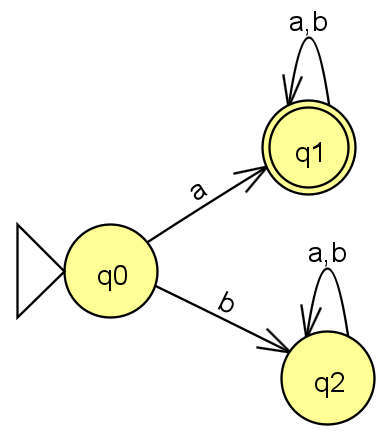
\includegraphics[width=0.2\textwidth]{../../../images/DFAs/ex1_q1.png}



% \vspace{3cm}
% \begin{flushleft}
% أرجو لكم وقتًا ممتعًا.

% الأستاذ محمود اغبارية.
% \end{flushleft}


% \end{document}


\ifwithsols
\title{حل اختبار فصلي \\ الصف العاشر 10}
\else
\title{اختبار فصلي \\ الصف العاشر 10}
\fi

\begin{document}

\maketitle

\begin{flushleft}
    $02.06.2026$
\end{flushleft}

\ifwithsols
\else
\begin{boxCode}
    \begin{itemize}
        \item يحتوي الاختبار على 4 أسئلة، \textbf{أجب عنها كلّها} $(4 \times 25 = 100)$.
        \item الوقت المخصص: ساعتان.
        \item يسمح باستخدام كل مادة مساعدة، عدا الآلة التي يمكن برمجتها.
        \item اكتب بقلم حبر فقط، وبخط واضح.
        \item الحل على ورقة خارجية، لا تنسَ كتابة اسمك.
    \end{itemize}
\end{boxCode}

\begin{center}
  
\includegraphics[width=0.4\textwidth]{../../../images/logoTasamoh.png}
\end{center}

\vspace{2cm}
\begin{flushleft}
    أرجو لكم التفوّق.

    الأستاذ محمود اغبارية.
\end{flushleft}
\clearpage
\fi

%%%%%%%%%%%%%%%%%%%%%%%%%%%%%%%%%%%%
\subsection*{السؤال الأول}
أمامك العملية \textenglish{What} التالية:

\begin{boxCode}
\begin{english}
\begin{minted}{csharp}
public static int What(int[] arr)
{
    int y = 0;
    int x = arr[0];
    for (int i = 0; i < arr.Length; i++)
    {
        y += arr[i];
        x = Math.Max(x, y);
        y = Math.Max(y, 0);
    }
    return x;
}
\end{minted}
\end{english}
\end{boxCode}

معطاة المصفوفة \textenglish{arr}:

{\small
\begin{english}
\begin{center}
\renewcommand{\arraystretch}{1.5}
\setlength{\tabcolsep}{12pt}
\begin{tabular}{c | c | c | c | c | c | c |}
\multicolumn{1}{c}{} & \multicolumn{1}{c}{0} & \multicolumn{1}{c}{1} & \multicolumn{1}{c}{2} & \multicolumn{1}{c}{3} & \multicolumn{1}{c}{4} & \multicolumn{1}{c}{5} \\
\cline{2-7}
\textenglish{arr} & $3$ & $4$ & $-8$ & $10$ & $-6$ & $8$ \\
\cline{2-7}
\end{tabular}
\end{center}
\end{english}
}

تتبّعوا، بواسطة جدول متابعة، العمليّة \textenglish{What(arr)}، واكتبوا ماذا تُعيد العمليّة. \\
يجب أن يشمل جدول المتابعة عمودًا لكلّ واحد من المتغيّرات التّالية: \textenglish{i, y, x}.

\ifwithsols
\begin{boxSolution}
\renewcommand{\arraystretch}{1.2}
\begin{tabular}{|c|c|c|c|}
\hline
\textenglish{i} & \textenglish{y} & \textenglish{x} \\
\hline
 & 0 & 3 \\
\hline
0 & 3 & 3 \\
\hline
1 & 7 & 7 \\
\hline
2 & 0 & 7 \\
\hline
3 & 10 & 10 \\
\hline
4 & 4 & 10 \\
\hline
5 & 12 & 12 \\
\hline
\end{tabular}
\vspace{1em} \\
\textbf{تعيد العملية:} \textenglish{12}
\end{boxSolution}
\fi

%%%%%%%%%%%%%%%%%%%%%%%%%%%%%%%%%%%%%%%%%%%%%%%%%%%%%%%%%%%%%%%%%%%%%%%%%%%%%%%%%%%%%%%%%%%%%%%%%%%%%%%
\clearpage
\subsection*{السؤال الثاني}
تُعرّف "\textbf{المصفوفة المتموجة}" بأنها مصفوفة تتناوب فيها حالة الترتيب بين كل حدين متجاورين باستمرار، صعوداً وهبوطاً:
\begin{itemize}
  \item إذا بدأت المصفوفة \textbf{بتصاعد} (الحد الأول أصغر من الحد الثاني)، فيجب أن يتبعه \textbf{هبوط} (الحد الثاني أكبر من الثالث)، ثم \textbf{تصاعد} (الثالث أصغر من الرابع)، وهكذا دواليك.
  \item أما إذا بدأت المصفوفة \textbf{بهبوط} (الحد الأول أكبر من الثاني)، فيجب أن يتبعه \textbf{تصاعد} (الثاني أصغر من الثالث)، ثم \textbf{هبوط} (الثالث أكبر من الرابع)، وهكذا.
  \item يُمنع وجود حدين متجاورين متساويين، ويُمنع وجود حالتي صعود متتاليتين أو حالتي هبوط متتاليتين.
\end{itemize}

اكتب عملية خارجية باسم \textenglish{IsWavy}، تتلقى مصفوفة من نمط صحيح \textenglish{arr}.
وتعيد العملية \textenglish{true} إذا كانت المصفوفة المتلقاة "متموجة"، وخلاف ذلك تعيد \textenglish{false}. \\
افترض أن كبر المصفوفة هو 3 على الأقل.

\textbf{أمثلة:}
\begin{itemize}
  \item بالنسبة للمصفوفة \textenglish{[2, 7, 4, 8, 3, 5]}، تعيد العملية \textenglish{true}.\\
  \textbf{الشرح:} العلاقة بين الحدود تتناوب باستمرار: تصاعد (2 أصغر من 7)، هبوط (7 أكبر من 4)، تصاعد (4 أصغر من 8)، هبوط، تصاعد.

  \item بالنسبة للمصفوفة \textenglish{[9, 5, 8, 1, 4]}، تعيد العملية \textenglish{true}.\\
  \textbf{الشرح:} العلاقة بين الحدود تتناوب باستمرار: هبوط (9 أكبر من 5)، تصاعد (5 أصغر من 8)، هبوط، تصاعد.

  \item بالنسبة للمصفوفة \textenglish{[2, 5, 7, 3]}، تعيد العملية \textenglish{false}.\\
  \textbf{الشرح:} المسار المتموج ينكسر في البداية بسبب وجود حالتي تصاعد متتاليتين (2 أصغر من 5، و 5 أصغر من 7).

  \item بالنسبة للمصفوفة \textenglish{[4, 4, 2, 5]}، تعيد العملية \textenglish{false}.\\
  \textbf{الشرح:} يوجد حدان متجاوران متساويان (4 و 4).
\end{itemize}

\ifwithsols
يمكن حل هذا السؤال بعدة طرق، لأنّه يمكن التعبير عن الشرط المطلوب بعدة طرق مكافئة
\begin{boxSolution}[الطريقة الأولى]
\begin{english}
\begin{minted}{csharp}
public static bool IsWavy(int[] arr)
{
    if (arr[0] == arr[1])
        return false;

    bool isGoingUp = arr[0] < arr[1];

    for (int i = 1; i < arr.Length - 1; i++)
    {
        if (isGoingUp)
        {
            if (arr[i] <= arr[i+1])
                return false;
            isGoingUp = false;
        }
        else
        {
            if (arr[i] >= arr[i+1])
                return false;
            isGoingUp = true;
        }
    }
    return true;
}
\end{minted}
\end{english}
\end{boxSolution}
\begin{boxSolution}[الطريقة الثانية]
    يمكننا التأكد من الشرط المطلوب عن طريق التأكد أنّه لا يوجد حد معين أصغر من جاريه أو أكبر من جارَيه المجاورين. \\
    أو بكلمات أخرى: لا يوجد 3 حدود متتالية تمثل متوالية تصاعدية أو تنازلية. \\
    انتبه لحدود $i$ في الحلقة.
\begin{english}
\begin{minted}{csharp}
public static bool IsWavy(int[] arr)
{
    for (int i = 1; i < arr.Length - 1; i++)
    {
        if ((arr[i] >= arr[i - 1] && arr[i+1] >= arr[i]) ||
            (arr[i] <= arr[i - 1] && arr[i+1] <= arr[i]))
        {
            return false;
        }
    }
    return true;
}
\end{minted}
\end{english}
\end{boxSolution}
\fi

%%%%%%%%%%%%%%%%%%%%%%%%%%%%%%%%%%%%%%%%%%%%%%%%%%%%%%%%%%%%%%%%%%%%%%%%%%%%%%%%%%%%%%%%%%%%%%%%%%%%%%%%
\clearpage
\subsection*{السؤال الثالث}

معطى عدد صحيح وأكبر من 0. \\
\textbf{خَلْط} عدد هو عدد \underline{آخر} بنفس الطول، مكوّن من نفس الأرقام المكوّن منها العدد الحاليّ، لكن بترتيب آخر. عدد مرّات ظهور كلّ رقم في العدد الحاليّ يساوي عدد مرّات ظهور نفس الرقم في العدد الآخر. \\
مثال: العدد 21611. \\
\textbf{خَلْطان} ممكنان له هما العددان: 62111 ، 12116.

معطاة الفئة \textenglish{DigitStorage} التي تمثّل عددًا صحيحًا وأكبر من 0. للفئة صفة واحدة: \\
مصفوفة \textenglish{count} بكِبَر 10 من نمط صحيح. كلّ خليّة في المصفوفة تحوي عدد مرّات ظهور الرقم في العدد الذي قيمة هذا الرقم فيه مساوية لقيمة مؤشّر (إندكس) الخليّة. \\
مثال: بالنسبة للعدد 21611 تبدو المصفوفة \textenglish{count} على النحو التالي:

{\small
\begin{english}
\begin{center}
\renewcommand{\arraystretch}{1.5}
\setlength{\tabcolsep}{10pt}
\begin{tabular}{c | c | c | c | c | c | c | c | c | c | c |}
\multicolumn{1}{c}{} & \multicolumn{1}{c}{0} & \multicolumn{1}{c}{1} & \multicolumn{1}{c}{2} & \multicolumn{1}{c}{3} & \multicolumn{1}{c}{4} & \multicolumn{1}{c}{5} & \multicolumn{1}{c}{6} & \multicolumn{1}{c}{7} & \multicolumn{1}{c}{8} & \multicolumn{1}{c}{9} \\
\cline{2-11}
\textenglish{count} & 0 & 3 & 1 & 0 & 0 & 0 & 1 & 0 & 0 & 0 \\
\cline{2-11}
\end{tabular}
\end{center}
\end{english}
}
أمامك جزء من الفئة \textenglish{DigitStorage}:

\begin{english}
\begin{minted}{csharp}
public class DigitStorage
{
    private int[] count = new int[10];
}
\end{minted}
\end{english}

\begin{enumerate}[label=\textbf{(\Alph*)}]
    \item اكتب في الفئة \textenglish{DigitStorage}، عمليّة بنائيّة تتلقّى عددًا صحيحًا وأكبر من 0 وتبتدئ المصفوفة \textenglish{count} بحسب ذلك.

    \item اكتب في الفئة \textenglish{DigitStorage}، عمليّة داخليّة تتلقّى كائنًا \textenglish{other} من نمط \\ \textenglish{DigitStorage}. تُعيد العمليّة \textenglish{true} - إذا كان الكائن \textenglish{other} مطابقًا للكائن الحاليّ، خلاف ذلك - تُعيد العمليّة \textenglish{false}.

    \item اكتب عمليّة خارجيّة تتلقّى عددين صحيحين وأكبر من 0 ومختلفين. تُعيد العمليّة \textenglish{true} - إذا كان العددان \textbf{خَلْطَين}، خلاف ذلك - تُعيد العمليّة \textenglish{false}. عليك استعمال العمليّتين اللتين كتبتهما في البندين "أ" وَ "ب".
\end{enumerate}

\ifwithsols
{\small
\begin{boxSolution}
\begin{english}
\begin{minted}{csharp}
class DigitStorage
{
    private int[] count = new int[10];

    // A
    public DigitStorage(int n)
    {
        while (n > 0)
        {
            this.count[n % 10]++;
            n /= 10;
        }
    }

    // B
    public bool IsIdentical(DigitStorage other)
    {
        for (int i = 0; i < 10; i++)
        {
            if (this.count[i] != other.count[i])
                return false;
        }
        return true;
    }
}

// C
public static bool IsPermutation(int n1, int n2)
{
    DigitStorage ds1 = new DigitStorage(n1);
    DigitStorage ds2 = new DigitStorage(n2);
    return ds1.IsIdentical(ds2);
}
\end{minted}
\end{english}
\end{boxSolution}
}
\fi

%%%%%%%%%%%%%%%%%%%%%%%%%%%%%%%%%%%%%%%%%%%%%%%%%%%%%%%%%%%%%%%%%%%%%%%%%%%%%%%%%%%%%%%%%%%%%%%%%%%%%%%%
\clearpage
\subsection*{السؤال الرابع}

أمامك واجهة الفئة \textenglish{Point} التي تمثّل نقطة في هيئة المحاور:

\begin{center}
\renewcommand{\arraystretch}{1.8}
{\small
\begin{tabular}{|p{0.5\textwidth}|l|}
\hline
\multicolumn{2}{|c|}{\textbf{\textenglish{Point}}} \\
\hline
صفة تُمثّل الإحداثي $x$ للنقطة في المستوى. & \textenglish{private double x} \\
\hline
صفة تُمثّل الإحداثي $y$ للنقطة في المستوى. & \textenglish{private double y} \\
\hline
عمليّة بنائيّة تتلقّى قيمًا لجميع صفات الكائن. & \textenglish{public Point(double x, double y)} \\
\hline
عمليّة تُعيد قيمة الإحداثي $x$. & \textenglish{public double GetX()} \\
\hline
عمليّة تُعيد قيمة الإحداثي $y$. & \textenglish{public double GetY()} \\
\hline
عمليّة تتلقّى كائنًا آخر من نمط \textenglish{Point} وتُعيد المسافة بين النقطة الحالية والنقطة الأخرى \textenglish{other}. \newline
(قانون المسافة: $d = \sqrt{(x_1 - x_2)^2 + (y_1 - y_2)^2}$) \newline
افترض أنّ \textenglish{other} ليس \textenglish{null}. & \textenglish{public double GetDistanceFrom(Point other)} \\
\hline
عمليّة تتلقّى كائنًا آخر من نمط \textenglish{Point} وتُعيد كائنًا \textbf{جديدًا} من نمط \textenglish{Point} يُمثّل نقطة المنتصف بين النقطة الحالية والنقطة الأخرى \textenglish{other}. \newline
(قانون نقطة المنتصف: $M = (\frac{x_1 + x_2}{2}, \frac{y_1 + y_2}{2})$) & \textenglish{public Point GetMiddlePoint(Point other)} \\
\hline
\end{tabular}
}
\end{center}

\begin{enumerate}[label=\textbf{(\Alph*)}]
    \item اكتب تطبيقًا كاملاً للفئة \textenglish{Point}:
\begin{enumerate}[label=\textbf{(\arabic*)}]
    \item اكتب تعريف الفئة مع الخصائص \textenglish{x} وَ \textenglish{y}.
    \item العمليّة البنائيّة وعمليّتي \textenglish{GetX} وَ \textenglish{GetY}.
    \item العمليّة \textenglish{GetDistanceFrom}.
    \item العمليّة \textenglish{GetMiddlePoint}.
\end{enumerate}
\begin{flushleft}
    انتبه: تكملة السؤال في الصفحة التالية
\end{flushleft}
\clearpage
\item اكتب عمليّة خارجية باسم \textenglish{GetMostRightPoint} تتلقى مصفوفة من نوع \textenglish{Point[]}.
تعيد العملية مؤشرًا من نوع \textenglish{Point} يُشير إلى النقطة الموجودة في أقصى اليمين في المستوى من بين النقاط التي في المصفوفة (أي النقطة التي لها أكبر إحداثي $x$ في المصفوفة).

% باسم \textenglish{IsValidTriangle}، تتلقى مصفوفة من نوع \textenglish{Point[]} تحتوي على ثلاث نقاط (أي بحجم 3).
%     تُعيد العملية \textenglish{true} إذا كانت هذه النقاط الثلاث يمكن أن تشكل رؤوس مثلث في المستوى، وخلاف ذلك تعيد \textenglish{false}.\\
%     تذكير رياضي: تشكل ثلاث نقاط مثلثاً إذا كان مجموع طولي أي ضلعين فيه أكبر من طول الضلع الثالث ($a+b>c$ وَ $a+c>b$ وَ $b+c>a$).

\item \textbf{(بونوس 10 علامات)} عمليّة باسم \textenglish{FindClosestPair}، تتلقى مصفوفة من نوع \textenglish{Point[]}.
    تقوم العملية بإيجاد أقرب نقطتين على بعضهما البعض في المصفوفة، وتطبع إحداثياتهما على الشاشة. \\
    افترض أن المصفوفة تحتوي على نقطتين على الأقل. \\
    \textbf{تلميح:} عليك استخدام حلقتين متداخلتين.

\end{enumerate}

\ifwithsols
{\small
\begin{boxSolution}[فرع أ]
\begin{english}
\begin{minted}{csharp}
public class Point
{
    private double x;
    private double y;

    public Point(double x, double y)
    {
        this.x = x;
        this.y = y;
    }

    public double GetX()
    {
        return this.x;
    }

    public double GetY()
    {
        return this.y;
    }

    public double GetDistanceFrom(Point other)
    {
        return Math.Sqrt(Math.Pow(this.GetX() - other.GetX(), 2)
                       + Math.Pow(this.GetY() - other.GetY(), 2));
    }

    public Point GetMiddlePoint(Point other)
    {
        double midX = (this.GetX() + other.GetX()) / 2;
        double midY = (this.GetY() + other.GetY()) / 2;
        Point middlePoint = new Point(midX, midY);
        return middlePoint;
    }
}
\end{minted}
\end{english}
\end{boxSolution}

\begin{boxSolution}[فرع ب + ج]
\begin{english}
\begin{minted}{csharp}
// B
public static Point GetMostRightPoint(Point[] arr)
{
    Point max = arr[0];
    for (int i = 1; i < arr.Length; i++)
    {
        if (arr[i].GetX() > max.GetX())
            max = arr[i];
    }
    return max;
}

// Bonus
public static void FindClosestPair(Point[] arr)
{
    double minDistance = double.MaxValue;
    Point p1 = null;
    Point p2 = null;

    for (int i = 0; i < arr.Length; i++)
    {
        for (int j = i + 1; j < arr.Length; j++)
        {
            double dist = arr[i].GetDistanceFrom(arr[j]);
            if (dist < minDistance)
            {
                minDistance = dist;
                p1 = arr[i];
                p2 = arr[j];
            }
        }
    }
    Console.WriteLine($"({p1.GetX()}, {p1.GetY()}) and ({p2.GetX()}, {p2.GetY()})");
}
\end{minted}
\end{english}
\end{boxSolution}
}
\fi

\end{document}
